\begin{frame}{Identification of Edge CFT}
\vskip-1.5cm
\newcommand{\uL}{\mathbf{L_0}}
\newcommand{\bL}{\mathbf{\bar{L}_0}}

\only<1>{
\begin{block}{Conformal Charge via 'Nested Entanglement Entropy'}
\vskip-0.5cm
	\begin{figure}[hbctp]
	\centering
	\includegraphics[width=0.8\textwidth]{{EdgeGS_EntanglementEntropy.pdf}}
	%\caption{Entanglement entropy within the entanglement ground state of the soft-core boson state on $10$ sites. For comparison, the Cardy-Calabrese formula $S(x) = c/3 \log \sin( \pi x/L) + const.$ is shown with $c=\frac{1}{2}, 1,$ and $2$, with the $const.$ fixed by matching the maximum of the entanglement entropy data. $c=1$ is a good fit.}
	%\label{fig:hc-edge-gs-ee}
	\end{figure}
	\begin{empheq}[box={\mybluebox[4pt][4pt]}]{equation*}
	c = 1
	\end{empheq}
\end{block}
}

\only<2>{
\begin{columns}[T]
\begin{column}{0.35\textwidth}

\begin{block}{Conformal Weights}
We can match the rescaled entanglement energies to the conformal weights of a free bosonic CFT.

%\begin{tabular*}{\columnwidth}{@{\extracolsep{\stretch{1}}}*{2}{c}@{}}
%\begin{tabularx}{\columnwidth}{|X|X|}
%\toprule
%\small
%\begin{align*}
%	\mathbf{P} &=&\frac{2\pi}{L}(\uL-\bL) 
%	&=& \frac{2\pi}{L}(em + n - \bar{n}) \\
%	%\widetilde{\mathbf{P}}&= em + n - \bar{n} &\\ 
%	\mathbf{H} &=& \frac{2\pi}{L}(\uL+\bL) 
%	&=& \frac{2\pi}{L}(\frac{\kappa e^2}{2} + \frac{m^2}{2 \kappa} + \frac{n + %\bar{n}}{2}) %\\
%\end{align*}
%\normalsize

%\begin{empheq}[box={\mybluebox[4pt][4pt]}]{equation*}
%\mathbf{H} \propto e^2 + \frac{m^2}{\kappa^2} + \frac{1}{\kappa}(n + \bar{n})
%\end{empheq}
$$
\mathbf{H} \propto e^2 + \frac{m^2}{\kappa^2} + \frac{1}{\kappa}(n + \bar{n})
$$
\end{block}
%}

%\only<3>{
\end{column}
\begin{column}{0.65\textwidth}
\begin{block}{Conformal primary identification in entanglement spectra}
\begin{figure}[hbctp]
\begin{center}
\includegraphics[width=\textwidth]{{EEIdentify.pdf}}
%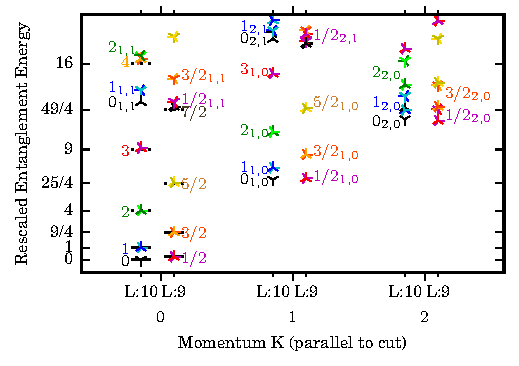
\includegraphics{{interpolatedboson/a10/plots/EEIdentify.pdf}}
\end{center}
%\caption{The identification of the states $\ket{e, m}_{n, \bar{n}}$ in the spectrum of the soft-core boson entanglement Hamiltonian. The label $e$ gives the U(1) charge. The labels $n$, $\bar{n}$ label the levels in the right or left-moving sectors of the Kac-Moody algebra. When the level $n$ is larger than 1, the level shows $Z(n)$ approximately degenerate states. The best estimate for the Luttinger parameter $\kappa = 1/6.4$ is given by the inverse of the energy of the $\ket{1, 0}_{1, 0}$ state. The label $m$ is 0 for all states shown - however, the primary states $\ket{e, m=\pm 1}$ can be seen centered around momentum $\pi$, with energies on the order of $1/(4\kappa^2)$.}
%\label{fig:primaries}
\end{figure}

\end{block}
\end{column}
\end{columns}
}

\end{frame}
